\pgfplotsset{compat=1.12}
\pgfplotsset{every tick label/.append style={font=\scriptsize}}
  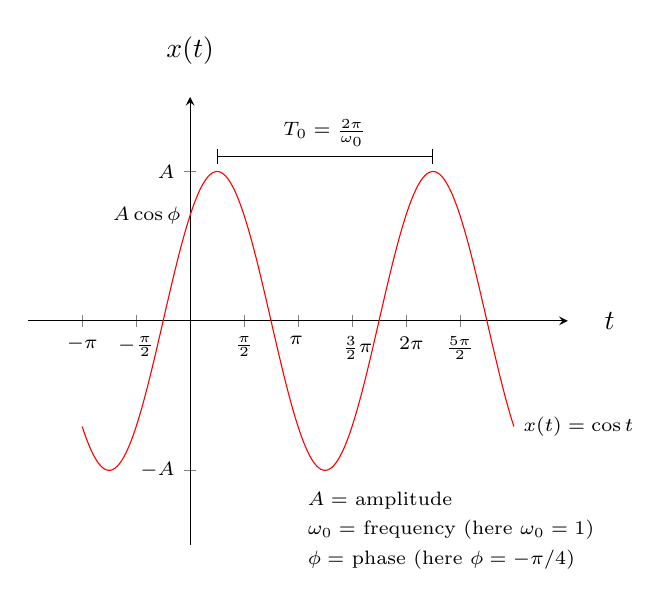
\begin{tikzpicture}
  \def\omwga0{2*pi}
  \def\phase{-45}
    \begin{axis}[
     clip=false,
     xmin=-1.5*pi,xmax=3.5*pi,
     xlabel= $t$,
     ylabel=$ x(t)$,
     ymin=-1.5,ymax=1.5,
     axis lines=middle,
     %axis x line=middle,
     %axis y line=left,
%     axis x line=middle,
     xtick={-3.14, -1.57, 0,1.57,3.14,4.71,6.28, 7.85},
     xticklabels={$-\pi$, $-\frac{\pi}{2}$, $0$, $\frac{\pi}{2}$,$\pi\,$,$\,\,\,\frac{3}{2}\pi$,$\,\,\,2\pi$, $\frac{5\pi}{2}$},
     ytick={-1, 1},
     yticklabels={$\small  -A$, $\small  A$},
     %xticklabel style={anchor=north west}
     every axis x label/.style={
    at={(ticklabel* cs:1.05)},
    anchor=west,
},
every axis y label/.style={
    at={(ticklabel* cs:1.05)},
    anchor=south,
},
     ]
      \addplot[domain=-pi:3*pi,samples=200,red]{cos(deg(x) + \phase)}
                                node[right,pos=1,font=\footnotesize, black]{\scriptsize $x(t)=\cos t$};


       \draw[|-|] (axis cs: pi/4,1.1) -- (axis cs: 2*pi +pi/4,1.1) node[midway, above] {\scriptsize $T_0=\frac{2\pi}{\omega_0}$};
       \node at (axis cs:0, .707) [anchor=east] {\scriptsize $A\cos\phi$  };

       \node at (axis cs:pi, -1.2) [anchor=west] {\scriptsize $A =$ amplitude };
       \node at (axis cs:pi, -1.4) [anchor=west] {\scriptsize $\omega_0 =$ frequency (here $\omega_0 =1$) };
       \node at (axis cs:pi, -1.6) [anchor=west] {\scriptsize $\phi =$ phase (here $\phi =-\pi/4$) };
    \end{axis}


  \end{tikzpicture} 